\chapter{Métricas de Software}
\label{chap:metricas}

\section{Processo de Medição}

Segundo o \citeonline{Guiaimplementacao}, a Medição apoia a gerência e a melhoria de processo e de produto, sendo um dos principais meios para gerenciar as atividades do ciclo de vida do trabalho e avaliar a viabilidade dos planos de trabalho. O propósito da Medição é coletar e analisar os dados relativos aos produtos desenvolvidos e aos processos implementados na organização e em seus trabalhos, de forma a apoiar o efetivo gerenciamento e demonstrar objetivamente a qualidade dos produtos \cite{ISO:12207}.

Ainda segundo o \citeonline{Guiaimplementacao}, entende-se por método de medição uma sequência lógica de operações, descritas genericamente, usadas para quantificar um atributo com respeito a uma escala especificada. Esta escala pode ser nominal, ordinal ou de razão (de proporção), bem como definida em um intervalo:

\begin{easylist}[itemize]	
	
	& \textbf{Nominal:} A ordem não possui significado na interpretação dos valores \cite{Meirelles2013}
	& \textbf{Ordinal:} A ordem dos valores possui significado, porém a distância entre os valores não. \cite{Meirelles2013}
	& \textbf{Intervalo:}  A ordem dos valores possui significado e a distância entre os valores também. Porém, a proporção entre os valores não necessariamente possui significado. \cite{Meirelles2013}
	& \textbf{Racional:} Semelhante a medida com escala do tipo intervalo, porém, a proporção possui significado. \cite{Meirelles2013}

	\end{easylist}

	
	A \citeonline{ISO:15939} também divide o processo de medição em dois métodos diferentes, que se distinguem pela natureza do que é quantificado:
	
	\begin{easylist}[itemize]

	& \textbf{Subjetiva:} Quantificação envolvendo julgamento de um humano.
	& \textbf{Objetiva:} Quantificação baseada em regras numéricas. Essas regras podem ser implementadas por um humano.

	\end{easylist}


%---------------------------------------------------------------------------------------------------------------------%

\section{Definição das métricas de software}

As métricas de software são medidas resultantes da medição do produto ou do processo do \textit{software} pelo qual é desenvolvido, sendo que o produto de \textit{software} deve ser visto como um objeto abstrato que se desenvolveu a partir de uma declaração inicial da necessidade de um sistema para um software finalizado, incluindo o código-fonte e as várias formas de documentação produzidas durante o desenvolvimento \cite{Mills:1999}. Estas medidas resultantes podem ser estudas para serem utilizadas para medir a produtividade e a qualidade do produto. 


\citeonline{Mills:1999} classifica as métricas de software como métricas de produtos ou métricas de processo, essa divisão pode ser vista na Figura \ref{modelodequalidade}. 

\begin{easylist}[itemize]	

& \textbf{Métricas de produtos:} são as medidas do produto de software em qualquer fase do seu desenvolvimento, a partir dos requisitos do sistema. Métricas de produto podem medir a complexidade da arquitetura do software, o tamanho do programa (código-fonte), ou o número de páginas de documentos produzidos. 

& \textbf{Métricas de processo:} são as medidas do processo de desenvolvimento de software, como o tempo de desenvolvimento global, o tipo de metodologia utilizada, ou o nível médio da experiência da equipe de programação.

\end{easylist}

\begin{figure}[h!]
\centering
\includegraphics[keepaspectratio=false,scale=0.65]{figuras/figuras_nilton/modeloqualidade.eps}
\caption{Modelo de Qualidade do Produto da \citeonline{ISO:9126}}
\label{modelodequalidade}
\end{figure}
\FloatBarrier

Na figura \ref{modelodequalidade} também pode ser notada a classificação das métricas de acordo com os diferentes tipos de medição, refletindo como as métricas influenciam nos contextos em que elas estão envolvidas. A qualidade do produto de software pode ser avaliada medindo-se os atributos internos (tipicamente medidas estáticas de produtos intermediários), os atributos externos (tipicamente pela medição do comportamento do código quando executado) ou os atributos de qualidade em uso \cite{ISO:9126}.

\begin{easylist}[itemize]

 & \textbf{Métricas internas:} Aplicadas em um produto de software não executável, como código fonte. Oferecem aos usuários, desenvolvedores ou avaliadores o benefício de poder avaliar a qualidade do produto antes que ele seja executável.
& \textbf{Métricas externas:} Aplicadas a um produto de software executável, medindo o comportamento do sistema do qual o software é uma parte através de teste, operação ou mesmo obervação. Oferecem aos usuários, desenvolvedores ou avaliadores o benefício de poder avaliar a qualidade do produto durante seu processo de teste ou operação.
& \textbf{Métricas de qualidade em uso:} Aplicadas para medir o quanto um produto atende as necessidades de um usuário para que sejam atingidas metas especificadas como eficácia, produtividade, segurança e satisfação.

\end{easylist}


%---------------------------------------------------------------------------------------------------------------------%

\section{Métricas de código fonte}
\label{sec:metricascodigo}

A definição de código-fonte segundo a SCAM é qualquer descrição executável de um sistema de software sendo incluído código de máquina, linguagens de alto nível e por representações gráficas executáveis \cite{harman}.

Segundo \citeonline{Mills:1999}, a maior parte do trabalho inicial em métricas de produto analisou as características do código-fonte. A partir da experiência com métricas e modelos, tornou-se cada vez mais evidente que as informações de métricas obtidas anteriormente do ciclo de desenvolvimento pode ser de grande valor no controle do processo e dos resultados, o que sucedeu uma série de trabalhos tratando sobre o tamanho ou complexidade do software. 

Neste capítulo, serão evidenciadas, em duas categorias as métricas de código-fonte que serão utilizadas neste trabalho de conclusão de curso, métricas de tamanho e complexidade e métricas de orientação a objetos. Estas métricas são objetivas e serão calculadas a partir da análise estática do código-fonte de um software. 

%--------------------------------------------
\subsection{Métricas de tamanho e complexidade}

Cada produto do desenvolvimento de software é uma entidade física, como tal, pode ser descrito em termos de tamanho. Desde outros objetos físicos são facilmente mensuráveis (em comprimento, volume, massa, ou outra medida padrão), medir o tamanho do software deve ser relativamente simples e coerente de acordo com os princípios da teoria da medição. No entanto, na prática, a medição de tamanho apresenta grandes dificuldades \cite{Fenton98}. 

Segundo \citeonline{honglei_research_2009}, as métricas de complexidade de  \textit{software} pertencem as principais medições de software e é o principal método para assegurar a qualidade do \textit{software}. Quanto menor a complexidade dos programas, melhor eles são, assim, as métricas de complexidade também podem ser usadas para prever os defeitos ou erros. A seguir são apresentadas algumas métricas de tamanho e complexidade.

\begin{easylist}[itemize]

	& \textbf{LOC} (\textit{Lines of Code}): Métrica simples em que são contadas as linhas executáveis de um código, desconsiderando linhas em branco e comentários.  \cite{metricsandmodels} 
		
	& \textbf{ACCM} (\textit{Average Cyclomatic Complexity per Method}): Mede a complexidade do programa, podendo ser representada através de um grafo de fluxo de controle. \cite{McCabe76}

	& \textbf{AMLOC} (\textit{Average Method Lines of Code}): Indica a distribuição de código entre os métodos. Quanto maior o valor da métrica, mais pesado é o método. É preferível que haja muitos métodos com pequenas operações do que um método grande e de entendimento complexo. \cite{Meirelles2013}
	
\end{easylist}

\subsection{Métricas de Orientação a Objetos}

Segundo \citeonline{budd_introduction_2002}, a programação orientada a objetos tornou-se extremamente popular nos últimos anos, inúmeros livros e edições especiais de revistas acadêmicas e comerciais têm surgido sobre o assunto. A julgar por essa atividade frenética, a programação orientada a objeto está sendo recebido com ainda mais entusiasmo do que vimos em ideias revolucionárias mais antigas, tais como programação estruturada "ou sistemas especialistas." 

Há uma série de razões importantes pelas quais, nas últimas duas décadas, a  
programação orientada a objetos tornou-se o paradigma de programação dominante. A programação orientada a objeto possui uma ótima escala, desde o mais trivial dos problemas para a maioria das tarefas complexas. Ele fornece uma forma de abstração que reflete em técnicas de como pessoas usam para resolver problemas em sua vida cotidiana. E para a maioria das linguagens orientadas a objeto dominante há um número cada vez maior de bibliotecas que auxiliam no desenvolvimento de aplicações para muitos domínios \cite{budd_introduction_2002}.

Serão adotadas neste trabalho as seguintes métricas de orientação a objetos:

\begin{easylist}
	
	%--------------------------
	& \textbf{ACC} (\textit{Afferent Connections per Class} - Conexões Aferentes por Classe): Mede a conectividade entre as classes. Quanto maior a conectividade entre elas, maior o potencial de impacto que uma alteração pode gerar. \cite{Meirelles2013}
	
	%--------------------------
	& \textbf{ANPM} (\textit{Average Number of Parameters per Method} - Média do Número de Parâmetros por Método): Indica a média de parâmetros que os métodos possuem. Um valor muito alto para quantidade de parâmetros pode indicar que o método está tendo mais de uma responsabilidade. \cite{Basili1987}

	%--------------------------
	& \textbf{CBO} (\textit{Coupling Between Objects} - Acoplamento entre Objetos): Essa é uma métrica que diz respeito a quantas outras classes dependem de uma classe. É a conta das classes às quais uma classe está acoplada. 		Duas classes estão acopladas quando métodos de uma delas utilizam métodos ou variáveis de outra. Altos 			valores dessa métrica aumentam a complexidade e diminuem a manutenibilidade.  \cite{softwaremeasurementandestimation}.
  		 
	%-----------------------------
	& \textbf{DIT} (\textit{Depth of Inheritance Tree} - Profundidade da 
	Árvore de Herança): Responsável por medir quantas camadas de herança compõem uma determinada hierarquia 		de classes \cite{softwaremeasurementandestimation}. Segundo \citeonline{Meirelles2013}, quanto maior o valor de DIT, maior o número de métodos e atributos herdados, portanto, maior a complexidade.

	%--------------------------
	& \textbf{LCOM4} (\textit{Lack of Cohesion in Methods} - Falta de Coesão
	entre Métodos): A coesão de uma classe é indicada por quão próximas as variáveis locais estão relacionadas com variáveis de instância locais. Alta coesão indica uma boa subdivisão de classes. A LCOM mede a falta de coesão através dissimilaridade dos métodos de uma classe pelo emprego de variáveis de instância.\cite{metricsandmodels}. A métrica LCOM foi revista e passou a ser conhecida como LCOM4, sendo necessário para seu cálculo a construção de um gráfico não-orientado em que os nós são os atributos e métodos de uma classe. Para cada método deve haver uma aresta entre ele e outro método ou variável. O valor da LCOM4 é o número de componentes fracamente conectados a esse gráfico \cite{Meirelles2013}

	%--------------------------
	& \textbf{NOC} (\textit{Number of Children} - Número de Filhos): É o número de sucessores imediatos,  (portanto filhos) de uma classe. Segundo \citeonline{softwaremeasurementandestimation}, altos valores indicam que a abstração da super classe foi diluída e uma reorganização da arquitetura deve ser considerada.
	
	%-----------------------------
	& \textbf{NOM} (\textit{Number of Methods} - Número de Métodos): Indica a quantidade de métodos de uma classe, medindo seu tamanho. Classes com muitos métodos são mais difíceis de serem reutilizadas pois são propensas a serem menos coesas. \cite{Meirelles2013}  

	%-----------------------------
	& \textbf{NPA} (\textit{Number of Public Attributes} - Número de Atributos Públicos): Mede o encapsulamento de uma classe, através da medição dos atributos públicos. O número ideal para essa métrica é zero \cite{Meirelles2013}

	%-----------------------------
	& \textbf{RFC} (\textit{Response For a Class} - Respostas para uma Classe): \citeonline{metricsandmodels} define essa métrica como o número de métodos que podem ser executados em respostas a uma mensagem recebida por um objeto da classe.

\end{easylist}	

%---------------------------------------------------------------------------------------------------------------------%

\section{Configurações de qualidade para métricas de código fonte} 

\citeonline{Meirelles2013} apresentou uma abordagem para a observação das métricas de código-fonte em seu doutorado, onde estas métricas foram estudadas através de suas distribuições e associações. Foram avaliados a distribuição e correlações dos valores das métricas de 38 projetos de software livre, sendo coletados e analisados valores para cada métrica em mais de 344.872 classes e módulos. Segundo o próprio \citeonline{Meirelles2013}, entre as principais contribuições de sua tese foi a análise detalhada, em relação ao comportamento, valores e estudos de caso, de 15 métricas de código-fonte. 

Dentre os objetivos científicos da tese de \citeonline{Meirelles2013} o mais crucial para este trabalho de conclusão de curso é o objetivo OC4, que trata das distribuições estatísticas dos valores de métricas em 38 projetos de software livre, a fim de compreender qual a abordagem estatística mais informativa para o monitoramento dessas métricas, bem como observar os valores frequentes para essas métricas, de forma a servirem de referência para projetos futuros.

\citeonline{Meirelles2013}, para conduzir o seu estudo quantitativo, utilizou-se da técnica de estatística descritiva: percentil. O percentil separa os dados em cem grupos que apresentam o mesmo número de valores, sendo a definição do percentil de ordem px100(0<p<1), em um conjunto de dados de tamanho n, é o valor da variável que ocupa a posição px(n+1) do conjunto de dados ordenados. O percentil de ordem p (ou p-quantil) deixa px100\% das observações abaixo dele na amostra ordenada. O percentil 25 recebe o nome de primeiro quartil, o percentil 50 de segundo quartil ou mediana, e o percentil 75 de terceiro quartil. Uma das hipóteses que \citeonline{Meirelles2013} utiliza é que só a partir do terceiro quartil será possível obter dados informativos sobre as métricas.

Após a aplicação da técnica percentil na série de dados das métricas de código-fonte obtidos da análise estática do código-fonte dos projetos de software livre, tabelas apresentando os valores percentis de cada métrica nos 38 projetos avaliados foram criadas, como a Tabela \ref{tab:percentil}, que mostra os percentis para a métrica NOC.  
	
	\begin{table}[!ht]
	\begin{center}
	
	\input{tabelas/tabelasNilton/percentis.ltx} 
	\caption{Percentis para métrica NOC em projetos Java extraídos de  
	\citeonline{Meirelles2013}}
	\label{tab:percentil}
	\end{center}
	\end{table}	
	\FloatBarrier	

Através dos resultados obtidos para cada métrica, \citeonline{Meirelles2013} observou que era possível identificar valores frequentes analisando os percentis. Na tabela \ref{tab:percentil}, por exemplo, considerando o projeto \textbf{Open JDK8} como referência, foram observados os intervalos de valores de 0, como muito frequente, 1 e 2 como frequente, 3 como pouco frequente e acima de 3 como não frequente \cite{Meirelles2013}. 

\citeonline{rego_monitoramento_2014}, observando o trabalho de análise de percentis de \citeonline{Meirelles2013}, percebeu que é possível utilizar os intervalos de frequência obtidos como uma evidência empírica de qualidade do código-fonte. \citeonline{rego_monitoramento_2014} também renomeou os intervalos de frequência obtidos por \citeonline{Meirelles2013}, como na Tabela \ref{tab:nomes}, a fim de facilitar a interpretação de métricas de código-fonte. 

\begin{table}[!ht]
	\begin{center}
	\input{tabelas/tabelasNilton/intervalos.ltx}
	\caption{Nome dos Intervalos de Frequência extraídos de \citeonline{rego_monitoramento_2014}}
	\label{tab:nomes}
	\end{center}
	\end{table}
	\FloatBarrier
	
\citeonline{rego_monitoramento_2014} observando a diferença dos valores das métricas entre os projetos analisados e na tentativa de diminuir tamanha diferença, considerou dois cenários. Foram utilizado dois produtos de \textit{software} como referências para cada uma das
métricas na linguagem de programação Java. Em um primeiro cenário, foi analisado o \textit{Open JDK8}, software que contia os menores valores percentis para as métricas. Já em um segundo cenário, foi considerado o Tomcat, contendo os valores percentis mais altos. A tabela \ref{tab:good-metrics} mostra o resultado desta análise:

\begin{table}[!ht]
	\begin{center}
	\input{tabelas/tabelasNilton/metricas.ltx}	
	\caption{Configurações para os Intervalos das Métricas para Java extraídas de \citeonline{rego_monitoramento_2014}}
	\label{tab:good-metrics}
	\end{center}
	\end{table}
	\FloatBarrier
   

%---------------------------------------------------------------------------------------------------------------------%

\section{Cenários de limpeza} 

Segundo \citeonline{marinescu2005measurement}, a utilização de métricas isoladas dificulta a interpretação de anomalias do código, reduzindo a aplicabilidade da medição feita. Além disso, o autor ainda afirma que a métrica por si só não contém informação suficiente para motivar uma transformação no código que melhore sua qualidade. Uma das soluções para sanar o problema da interpretação do código através de métricas isoladas é  interpretar o código através de cenários de limpeza.

\citeonline{Machini2010} apresenta uma maneira de interpretar os valores das métricas através de cenários problemáticos e suas possíveis melhorias, para que as métricas possam ser mais facilmente incorporadas no cotidiano dos programadores. \citeonline{Machini2010} também apresenta um estilo de programação baseado no paradigma da Orientação a Objetos que busca o que denominamos de “Código Limpo”, concebido e aplicado por renomados desenvolvedores de software como Robert C. Martin \cite{Martin2008} e Kent Beck \cite{Beck2007}	
	
Segundo \citeonline{Beck2007}, um código limpo está inserido em um estilo de programação que busca a proximidade a três valores: expressividade, simplicidade e flexibilidade.	

\begin{easylist}[itemize]

	& \textbf{Expressividade:} Um código se expressa bem quando alguém que o lê é capaz de compreendê-lo e modificá-lo. \citeonline{Beck2007} destaca que quando foi necessário modificar um código, ele gastou muito mais tempo lendo o que já havia sido feito do que escrevendo sua modificação. 
		
	& \textbf{Simplicidade:} Um código é simples quando pode ser facilmente lido, havendo uma redução da quantidade de informação que o leitor deve compreender para fazer alterações. Eliminar o excesso de complexidade faz com que aqueles que estejam lendo o código o entenda mais rapidamente. 

	& \textbf{Flexibilidade:} Capacidade de estender a aplicação alterando o mínimo possível a estrutura já criada.
		
\end{easylist}

\citeonline{Machini2010} apresenta em seu trabalho diversas técnicas para a obtenção de um código limpo. Um resumo destas técnicas são apresentadas nas tabelas \ref{tab:conceitos1}, \ref{tab:conceitos2}, \ref{tab:conceitos3} e \ref{tab:conceitos4}.


\begin{table}[!ht]
\centering
\input{tabelas/tabelasNilton/conceitos-limpeza-parte1.ltx}
\caption{Conceitos de Limpeza levantados por \citeonline{Machini2010} e adaptados por \citeonline{rego_monitoramento_2014} parte 1.}
\label{tab:conceitos1}
\end{table}
\FloatBarrier

\begin{table}[!ht]
\centering
\input{tabelas/tabelasNilton/conceitos-limpeza-parte2.ltx}
\caption{Conceitos de Limpeza levantados por \citeonline{Machini2010} e adaptados por \citeonline{rego_monitoramento_2014} parte 2.}
\label{tab:conceitos2}
\end{table}
\FloatBarrier

\begin{table}[!ht]
\centering
\input{tabelas/tabelasNilton/conceitos-limpeza-parte3.ltx}
\caption{Conceitos de Limpeza levantados por \citeonline{Machini2010} e adaptados por \citeonline{rego_monitoramento_2014} parte 3.} 
\label{tab:conceitos3}
\end{table}
\FloatBarrier

\begin{table}[!ht]
\centering
\input{tabelas/tabelasNilton/conceitos-limpeza-parte4.ltx}
\caption{Conceitos de Limpeza levantados por \citeonline{Machini2010} e adaptados por \citeonline{rego_monitoramento_2014} parte 4.} 
\label{tab:conceitos4}
\end{table}
\FloatBarrier

Após apresentar as técnicas para obtenção de um código limpo, \citeonline{Machini2010}   adota uma abordagem baseada em cenários para identificar trechos de código com características indesejáveis. Os cenários devem possuir um contexto criado a partir de poucos conceitos de código limpo no qual um pequeno conjunto de métricas é analisado e interpretado através da combinação de seus valores. A ideia principal desta abordagem é facilitar melhorias de implementação e a procura por problemas quanto a limpeza de código através da aproximação dos valores das métricas com os esperados nos contextos de interpretação \cite{Machini2010}.

\citeonline{rego_monitoramento_2014} utiliza a mesma abordagem de cenários que \citeonline{Machini2010}, onde algumas técnicas de limpeza de código apresentadas nas tabelas \ref{tab:conceitos1}, \ref{tab:conceitos2}, \ref{tab:conceitos3} e \ref{tab:conceitos4} são correlacionadas com as métricas da Seção \ref{sec:metricascodigo}. Adicionalmente, utiliza-se a configuração do \textit{ Open JDK8 } considerando como valores altos os valores obtidos pelos intervalos Regular e Ruim tal como mostrados na Tabela \ref{tab:good-metrics}.

Aproveitando inicialmente os cenários \textbf{Classe pouco coesa} e \textbf{Interface dos métodos} extraídos de  \citeonline{Machini2010}, \citeonline{rego_monitoramento_2014} elaborou mais alguns cenários de limpeza. O resultado dessa atividade pode ser visto na tabela \ref{tab:cenarios}:

\begin{sidewaystable}
\begin{table}[H]
\centering
\input{tabelas/tabelasNilton/cenarios.ltx}
\caption{Cenários de Limpeza extraídos de \citeonline{rego_monitoramento_2014}}
\label{tab:cenarios}
\end{table}
\FloatBarrier
\end{sidewaystable}  

\section{Considerações Finais do Capítulo}  

Esse capítulo apresentou a fundamentação teórica sobre métricas de código fonte, quais são seus intervalos qualitativos e também foi apresentada a maneira como elas foram relacionadas a cenários de limpeza. O próximo capítulo será responsável por apresentar a importância dos Verificadores Estáticos de Código.

